Al comienzo de este Trabajo de Fin de Grado, se organizan las tareas de
forma coherente, definiendo cada procedimiento. Sin embargo, los
conflictos encontrados a la hora de disponer de la herramienta
\emph{Star CCM+}, supuso un cambio de planteamiento, sustituyendo esta
herramienta comercial por la alternativa libre \emph{OpenFOAM}.

Tras consultar a algún profesor, conocedor de la herramienta, por la
viabilidad de utilizarlo en este estudio, confirman las garantías del
código. También, advirten que es un software muy completo pero complejo.
El cual exige una curva de aprendizaje notable e implica adquirir
ciertos conocimientos en ingeniería de software, trabajar con sistemas
operativos de Linux y no tener barreras para trabajar por línea de
comandos.

A continuación se presenta un diagrama donde se resumen las fases
desarrolladas para abordar un problema de dinámica de fluidos a través
de \emph{OpenFOAM}:\\

\begin{figure}
\centering
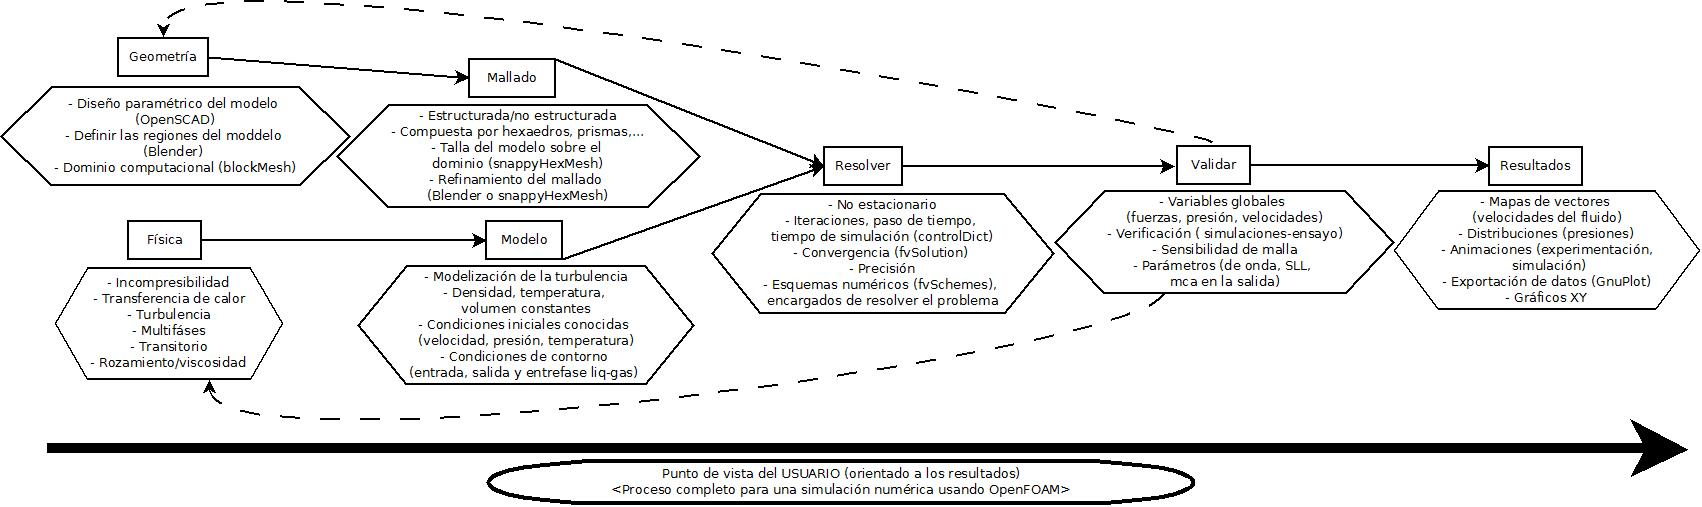
\includegraphics[width=\linewidth]{21-ProcesoTFG.jpg}
\caption[Diagrama de proceso]{Diagrama de proceso completo para una simulación
numérica usando OpenFOAM}
\label{fig:ProcesoTFG}
\end{figure}

Teniendo una idea de cómo proceder con las simulaciones, se realizará el
estudio de selección de un prototipo para el aprovechamiento de la
energía undimotriz. Se prosigue con la fabricación de la maqueta para la
experimentación en el laboratorio de fluidos de la escuela. Y para
finalizar, se realiza una comparación de los resultados de las
simulaciones por ordenador, con las mediciones reales ensayadas.

Entonces, las tareas a completar para la elaboración del proyecto se
pueden desglosar en las siguientes:

\begin{table}
\centering
\caption{Proceso del proyecto}
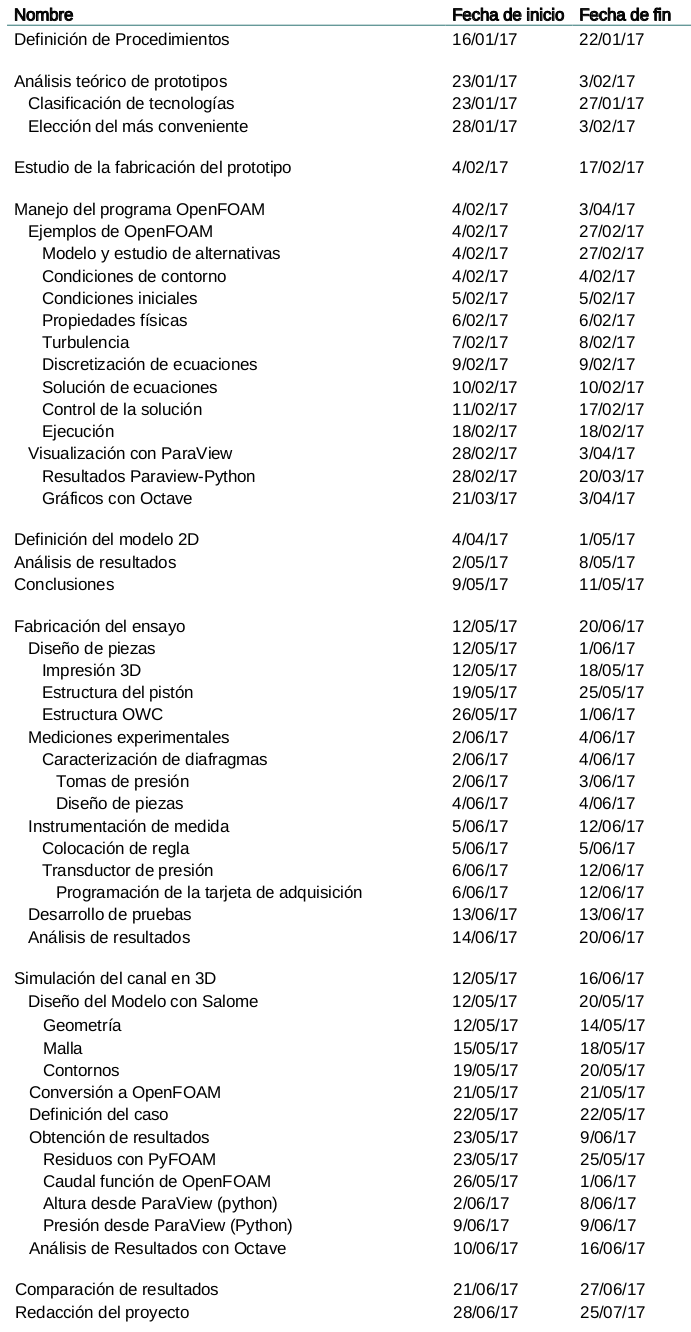
\includegraphics{21-GanttTareas.png}
\end{table}

De la tabla anterior se obtienen un total de 52 tareas a realizar entre
el 16 de enero de 2017 y el 26 de julio de 2017. Asimismo, en la
siguiente imagen se representa el diagrama de estas tareas:

\begin{figure}
\centering
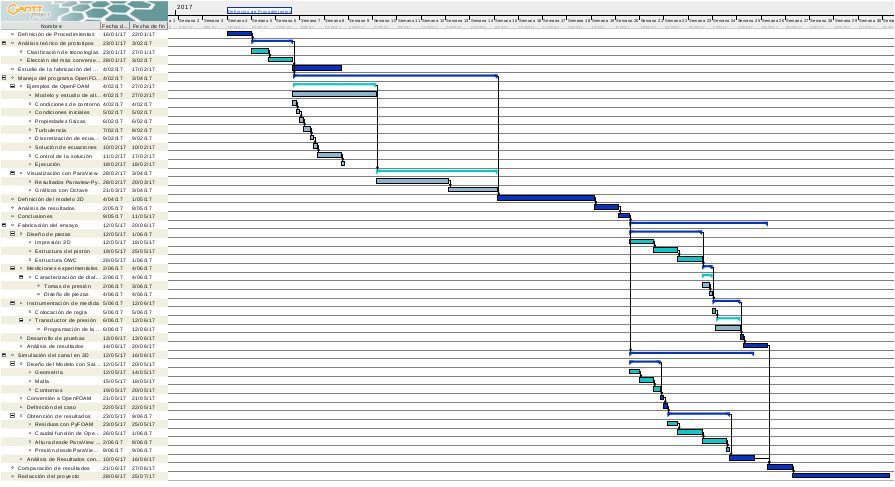
\includegraphics[width=\linewidth]{22-GanttDiagrama.png}
\caption{Diagrama de Gantt del proceso del proyecto}
\label{fig:GanttDiagrama}
\end{figure}

Los plazos establecidos son orientativos, ya que tanto en alguna de las
tres fases de las simulaciones (preproceso, procesado y postproceso),
como en las adaptaciones del ensayo, es muy probable encontrarse con
dificultades. Además, dada la temprana madurez de estas técnicas la
información, a veces, resulta difícil de encontrar y, en otras, se da
con la solución por prueba y error.
